\section{\texthebrew{תקציר}}

\begin{hebrew}מטרת מחקר זה היא לבחון כיצד פיגמנטים תזונתיים משנים את צבע הצואה ופרמטרים צואתיים נוספים. פיתחנו מודל מאוחד פרמקוקינטי (\textenglish{pharmacokinetic}) וקולורימטרי להערכת השפעת הפיגמנטים על הכרומטיקה של הצואה, ובכלל זה מדד רב-משתני לכרומטיקה צואתית (\textenglish{Faecal Chromatics Index, FCI}) המשלב מדידות צבע לפי \textenglish{CIEDE2000}, מרקם לפי סולם הצואה של \textenglish{Bristol}, חומציות צואתית (\textenglish{pH}) וזמן מעבר לומינלי. המודל שלנו מצביע כי ה-\textenglish{betalains} מצריכת סלק עשויים לחולל שינויים ניכרים בצבע הצואה — תופעה המכונה \textenglish{beeturia} — תוך השפעה גם על רמת ה-\textenglish{pH} הצואתית. עבודה זו מספקת מסגרת מקיפה להבנת יחסי הגומלין המורכבים שבין התזונה לבין מאפייני הצואה.\end{hebrew}

\section{\texthebrew{מבוא}}

\begin{hebrew}הערכת מאפייני הצואה משמשת ככלי אבחוני לא-פולשני חיוני בפרקטיקה הקלינית. צבע הצואה ומרקמה מספקים רמזים חזותיים מיידיים העשויים להעיד על מצבים שונים במערכת העיכול, החל מהשפעות תזונתיות ועד לפתולוגיות חמורות יותר \cite{beeturia}. ואולם, ההסתמכות הנוכחית על הערכות איכותניות של פרמטרים אלו נתונה לשונות ניכרת וחסרה את הדיוק הנדרש לאבחון ולניטור מהימנים של בריאות מערכת העיכול.\end{hebrew}

\begin{hebrew}פיגמנטים תזונתיים, כגון ה-\textenglish{betalains} המצויים בסלק, עשויים לצבוע באופן נראה את הצואה, ולגרום לתופעה הידועה בשם \textenglish{beeturia}. ה-\textenglish{betalains} הם פיגמנטים מסיסים במים המתפקדים ככרומופורים, ומשווים גוון אדום או סגול אופייני לצואה \cite{beeturia}. השפעה זו בולטת במיוחד בתנאים של הפרשת חומצה קיבתית מופחתת וצמחיית מעיים משתנה, ומדגישה את יחסי הגומלין המורכבים שבין הצריכה התזונתית לבין תפקוד מערכת העיכול.\end{hebrew}

\begin{figure}[h]\centering
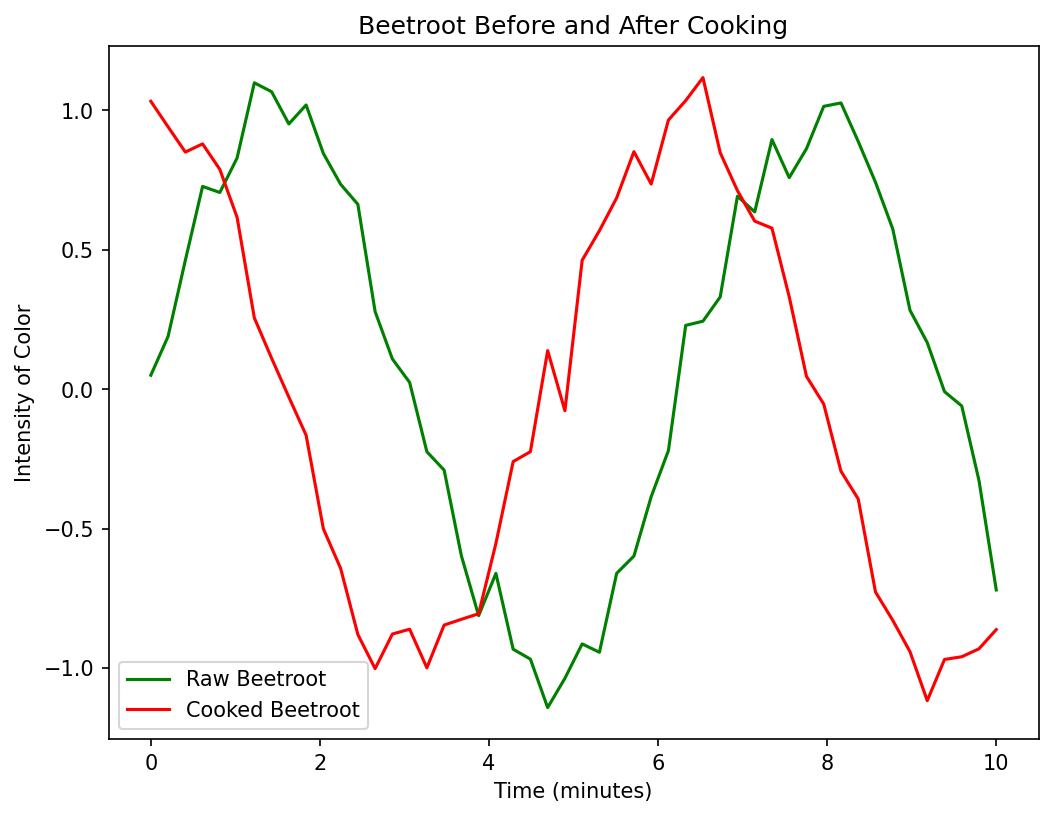
\includegraphics[width=0.9\textwidth]{../assets/F1.png}
\caption{\texthebrew{סלק נא ומבושל — מקור ה-\textenglish{betacyanin} הנחקר.}}
\end{figure}

\begin{hebrew}חרף הרלוונטיות הקלינית, הערכת מאפייני הצואה נותרה במידה רבה איכותנית. אופיין הסובייקטיבי של הערכות אלו מכניס שונות ניכרת בין מעריכים, ובכך מגביל את התועלת האבחונית שלהן \cite{beeturia}. כדי להתמודד עם מגבלה זו, אנו מציעים מסגרת כמותית רב-משתנית המשלבת את צבע הצואה, המרקם, ה-\textenglish{pH} וזמן המעבר הלומינלי.\end{hebrew}

\begin{hebrew}המודל שלנו מציע כי שילובם של ניתוח ספקטרופוטומטרי לצבע הצואה, סיווג מרקם לפי סולם \textenglish{Bristol Stool Scale (BSS)}, מדידת חומציות צואתית, ומידול פרמקוקינטי לזמן המעבר — יציע מערכת הערכה מקיפה. תרומות עבודה זו הן: (1) מעבר מהערכה איכותנית לכמותית; (2) מדד \textenglish{FCI} מאוחד; (3) רלוונטיות קלינית להתאמת המלצות תזונה; ו-(4) קידום מתודולוגי במדידת כרומטיקה צואתית.\end{hebrew}

\begin{hebrew}מעבר לערך האבחוני, כימות מאפייני הצואה פותח אפשרויות למחקר אפידמיולוגי רחב-היקף: באמצעות מדדים אובייקטיביים ניתן להשוות בין אוכלוסיות, לעקוב אחר שינויים לאורך זמן, ולשלב את הנתונים במערכות ניטור ביתיות. גישה כמותית כזו אף מצמצמת את התלות בזיכרון הנבדק או בדיווח עצמי — מקור שכיח להטיה במחקרי תזונה — ומאפשרת איסוף נתונים בקנה מידה גדול ללא מאמץ מצד המשתתפים.\end{hebrew}

\begin{hebrew}לסיכום, מחקר זה מבקש לעודד מעבר להערכה כמותית של מאפייני הצואה ככלי אבחון לא-פולשני, תוך איחוד צבע, מרקם, \textenglish{pH} וזמן מעבר במסגרת אחת.\end{hebrew}

\section{\texthebrew{סקירת ספרות}}

\begin{hebrew}תופעת ה-\textenglish{beeturia} — שינוי צבע ההפרשה בעקבות צריכת סלק — תועדה כבר באמצע המאה ה-20, ומחקרים מוקדמים אמדו את שכיחותה בקרב האוכלוסייה בכ-10\%--14\% \cite{beeturia}. עבודות אלו התמקדו בעיקר בשתן, אך הצביעה הצואתית — נושא מחקרנו — נחקרה פחות באופן כמותי, חרף היותה אינדיקטור נגיש ושכיח.\end{hebrew}

\begin{hebrew}הכימיה של ה-\textenglish{betalains} נחקרה בהרחבה: סקירות מקיפות תיארו את המבנה האינדולי, את ההבחנה בין \textenglish{betacyanins} ל-\textenglish{betaxanthins}, ואת יציבותם התלויה ב-\textenglish{pH} ובטמפרטורה \cite{betalain}. ממצאים אלו רלוונטיים ישירות לשאלה כיצד שורד ה-\textenglish{betanin} את המעבר במערכת העיכול ומגיע אל הצואה תוך שמירה על גוון אדום.\end{hebrew}

\begin{hebrew}בתחום הקולורימטריה, מרחב הצבע \textenglish{CIELAB} ותקני ה-\textenglish{CIE} מספקים בסיס סטנדרטי לכימות צבע \cite{cie2004}. נוסחת הפרש הצבע \textenglish{CIEDE2000} שכללה את המדידה באמצעות פונקציות שקלול תפיסתיות ואיבר סיבוב, והפכה לסטנדרט המקובל להערכת הפרשי צבע הנתפסים על ידי הראייה האנושית \cite{ciede2000}. אנו מאמצים מסגרת זו לכימות אובייקטיבי של צבע הצואה.\end{hebrew}

\begin{hebrew}המידול הפרמקוקינטי של ספיגה וסילוק מסדר ראשון מבוסס היטב בספרות הקלאסית \cite{rowland2011}, ומספק את הכלים לתיאור פרופיל הריכוז הלומינלי לאורך זמן. אנו מיישמים עקרונות אלו על מעבר הפיגמנט במעי, תוך קישור בין הפרמקוקינטיקה לבין הצביעה הנצפית.\end{hebrew}

\begin{hebrew}הערכת מרקם הצואה זכתה לתקינה באמצעות \textenglish{Bristol Stool Scale}, שהפך לכלי הקליני המקובל לסיווג צורת הצואה לשבעה טיפוסים ולהיסק על זמן המעבר. שילוב סולם זה עם מדידות צבע, \textenglish{pH} וזמן מעבר הוא לב הגישה הרב-משתנית שלנו.\end{hebrew}

\begin{hebrew}לבסוף, התפתחות טכנולוגיות הניטור הביתי — ובכללן מערכות אסלה חכמה (\textenglish{smart toilet}) וחיישנים ספקטרופוטומטריים לבישים — פותחת אפשרות לקולורימטריה צואתית בזמן אמת \cite{park2020}. עבודתנו מספקת את הבסיס הכמותי הדרוש לפרשנות אוטומטית של נתונים אלו, ובכך מגשרת בין הספרות הביוכימית, הקולורימטרית והקלינית הקיימת לבין יישומים עתידיים.\end{hebrew}

\section{\texthebrew{רקע: כימיה של פיגמנטים}}

\begin{hebrew}צביעת הצואה האנושית נובעת מפיגמנטים תזונתיים השורדים את המעבר במערכת העיכול ותורמים לגוון הצואה. פרק רקע זה סוקר את הכרומופורים העיקריים האחראים לצביעה הצואתית ואת יציבותם בתנאים הפיזיולוגיים בכרכשת (\textenglish{colon}).\end{hebrew}

\subsection{\texthebrew{מחלקות כרומופורים}}

\begin{hebrew}מספר מחלקות של פיגמנטים תזונתיים ידועות כמשפיעות על צבע הצואה: \textenglish{betalains}, \textenglish{anthocyanins}, \textenglish{chlorophylls}, \textenglish{carotenoids} וצבעי \textenglish{azo}. לכל מחלקה תכונות כימיות נבדלות הקובעות את יכולתה לשרוד את המעבר במעי ולהקנות צבע לצואה.\end{hebrew}

\begin{figure}[h]\centering
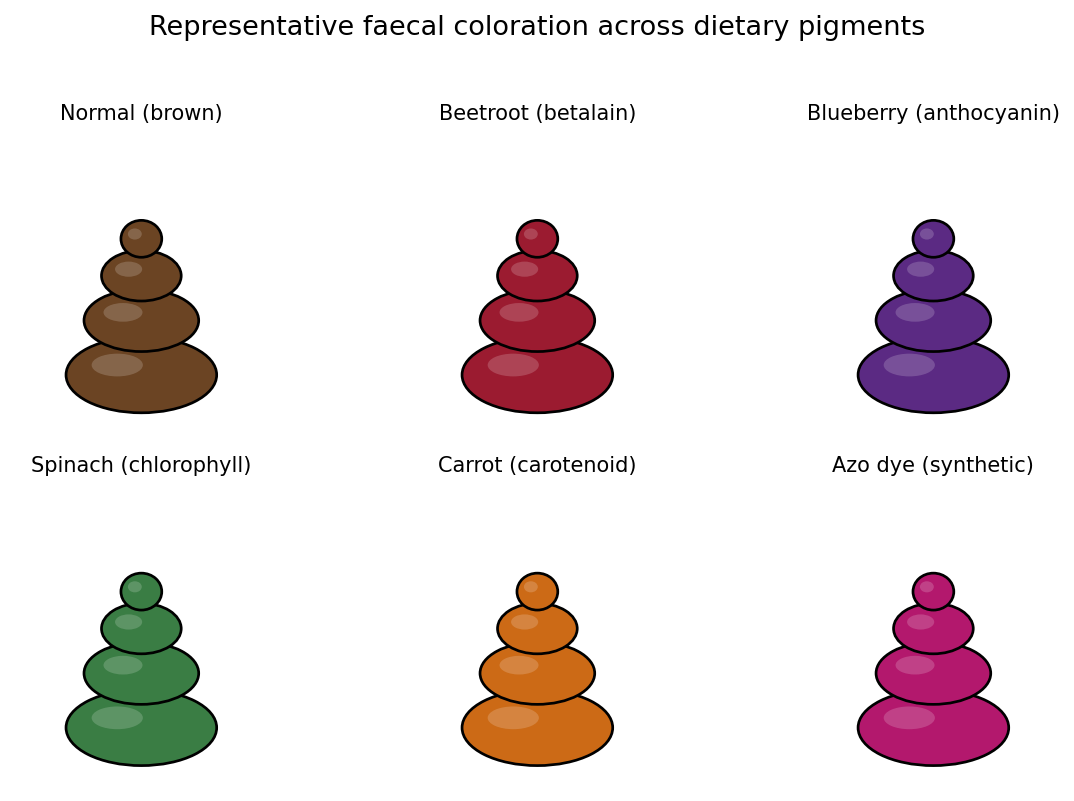
\includegraphics[width=0.9\textwidth]{../assets/F10.png}
\caption{\texthebrew{צביעה צואתית ייצוגית על פני פיגמנטים תזונתיים שונים.}}
\end{figure}

\begin{hebrew}\textbf{\textenglish{Betalains}.} ה-\textenglish{betalains}, המצויים בעיקר בסלק (\textenglish{Beta vulgaris}) ובצמחים נוספים מסדרת ה-\textenglish{Caryophyllales}, הם תרכובות נגזרות-אינדול המאופיינות ב-\textenglish{betacyanins} אדומים-סגולים וב-\textenglish{betaxanthins} צהובים. ה-\textenglish{betacyanin} הנפוץ ביותר הוא ה-\textenglish{betanin}, המגלה יציבות פוטוכימית גבוהה אך יציבות תרמית בינונית. מבנהו הכימי הייחודי מאפשר לו לעמוד בפני פירוק אנזימטי במערכת העיכול, ולכן הוא שורד אל הצואה ומקנה לה צביעה אדומה אופיינית.\end{hebrew}

\begin{hebrew}\textbf{\textenglish{Anthocyanins}.} ה-\textenglish{anthocyanins} הם פיגמנטים ואקואולריים מסיסים במים האחראים לצבעים הכחולים, הסגולים והאדומים של פירות ופרחים. הם גליקוזידים של מולקולות \textenglish{anthocyanidin} בעלות מבנה כרומופורי בסיסי. ה-\textenglish{anthocyanins} מגלים יציבות משתנה בסביבות חומציות אך שורדים בדרך כלל את המעבר במעי בזכות עמידותם לאנזימים חיידקיים, ולכן תורמים לצביעת הצואה — בייחוד לאחר צריכת פירות יער.\end{hebrew}

\begin{hebrew}\textbf{\textenglish{Chlorophylls}.} ה-\textenglish{chlorophylls} הם הפיגמנטים הירוקים העיקריים בצמחים, האחראים לקליטת אנרגיית אור בפוטוסינתזה, ומבנם טבעת \textenglish{porphyrin} עם יון מגנזיום מרכזי. עם הבליעה הם עוברים מטבוליזם מהיר ל-\textenglish{pheophytins}, העשויים להקנות גוון ירוק לצואה. ה-\textenglish{chlorophylls} אינם יציבים יחסית במעי בשל רגישותם לתנאים חומציים ולפירוק אנזימטי.\end{hebrew}

\begin{hebrew}\textbf{\textenglish{Carotenoids}.} ה-\textenglish{carotenoids} הם פיגמנטי \textenglish{tetraterpenoid} האחראים לצבעים הצהובים, הכתומים והאדומים בפירות ובירקות, ובהם \textenglish{beta-carotene}, \textenglish{lycopene} ו-\textenglish{lutein}. הקשרים הכפולים המצומדים שבמולקולות אלו מאפשרים בליעת אור בטווחי אורך גל שונים. ה-\textenglish{carotenoids} מגלים יציבות גבוהה ומסוגלים לשרוד את המעבר ולתרום לצביעה הצואתית.\end{hebrew}

\begin{hebrew}\textbf{צבעי \textenglish{Azo}.} צבעי ה-\textenglish{azo} הם פיגמנטים סינתטיים הנפוצים בצביעת מזון ובתעשייה, ומכילים קבוצת \textenglish{azo} ($-N{=}N-$) ככרומופור המקנה גוונים עזים מצהוב עד אדום. תרכובות אלו שורדות את סביבת מערכת העיכול בזכות עמידותן לפירוק אנזימטי, אך עשויות להיות מושפעות משינויי \textenglish{pH}.\end{hebrew}

\subsection{\texthebrew{יציבות ה-\textenglish{betanin} ב-\textenglish{pH}}}

\begin{hebrew}יציבות ה-\textenglish{betanin} חשובה במיוחד בהקשר הצואתי. בתנאים חומציים מאוד ($pH < 3$) הוא עובר סידורים מבניים המפחיתים את עוצמת הצבע. עם זאת, בכרכשת — שבה ה-\textenglish{pH} גבוה יותר עקב תסיסה חיידקית (טווח אופייני $5.5$--$7.0$) — נשאר ה-\textenglish{betanin} יציב יחסית, וכך הוא נמשך אל הצואה ותורם לגוון האדום.\end{hebrew}

\subsection{\texthebrew{מנגנוני הפיגמנטציה הצואתית}}

\begin{hebrew}יכולתם של הפיגמנטים לשרוד את המעבר ולצבוע את הצואה מושפעת ממבנם הכימי, מעמידותם האנזימטית ומיציבותם ל-\textenglish{pH}. ה-\textenglish{betalains} וה-\textenglish{anthocyanins} עמידים במיוחד בזכות נוקשותם המבנית ורגישותם המוגבלת לאנזימים חיידקיים בכרכשת. ה-\textenglish{chlorophylls} וה-\textenglish{carotenoids} שורדים אף הם, אך עשויים לעבור פירוק חלקי במהלך המעבר. צבעי ה-\textenglish{azo} מגלים תכונות דומות אך רגישים יותר לתנאי הסביבה.\end{hebrew}

\subsection{\texthebrew{סיכום הכרומופורים}}

\begin{hebrew}הטבלה שלהלן מסכמת את הפיגמנטים העיקריים, מחלקת הכרומופור, השפעת הצביעה הצואתית, ופרמטרי הזמן והיציבות.\end{hebrew}

\begin{table}[h]\centering\small
\setlength{\tabcolsep}{4pt}
\begin{tabular}{lllllll}
\toprule
Food & Pigment Class & Chromophore & Stool Coloration & Onset (h) & Duration (h) & pH Stability \\
\midrule
Beets & Betalains & Betanin & Red & 4--6 & 12--24 & Stable (pH$>$3) \\
Berries & Anthocyanins & Anthocyanidins & Purple/Red & 2--4 & 8--16 & Variable \\
Spinach & Chlorophylls & Phylloquinone & Green & 2--3 & 4--8 & Unstable \\
Carrots & Carotenoids & Beta-carotene & Orange/Yellow & 1--2 & 6--12 & Stable \\
Artificial & Azo dyes & Azo group & Intense & Var. & Var. & pH-dependent \\
\bottomrule
\end{tabular}
\end{table}

\begin{hebrew}לסיכום, פיגמנטים תזונתיים כגון \textenglish{betalains}, \textenglish{anthocyanins}, \textenglish{chlorophylls}, \textenglish{carotenoids} וצבעי \textenglish{azo} ממלאים תפקיד מכריע בקביעת צבע הצואה דרך עמידותם לפירוק אנזימטי ויציבותם בתנאי \textenglish{pH} משתנים. הבנת מנגנונים אלו מספקת תובנה לפרמקוקינטיקה של ספיגת הפיגמנט והפרשתו במערכת העיכול.\end{hebrew}

\section{\texthebrew{פרמטרים של צואה וסולם בריסטול}}

\begin{hebrew}הערכת מאפייני הצואה משתרעת אל מעבר לבחינה חזותית גרידא, וכוללת פרמטרים שונים: מרקם, חומציות צואתית (\textenglish{pH}), תכולת מים וזמן מעבר. תכונות אלו, יחד, מספקות הבנה מקיפה של בריאות מערכת העיכול ותפקודה. סולם הצואה של \textenglish{Bristol} (\textenglish{Bristol Stool Scale}) הוא כלי מקובל לסיווג צורת הצואה לשבעה טיפוסים נבדלים, שלכל אחד מהם משמעות לגבי המעבר הלומינלי.\end{hebrew}

\subsection{\texthebrew{סולם הצואה של \textenglish{Bristol}}}

\begin{hebrew}הסולם מסווג את הצואה מטיפוס 1 (גושים קשים נפרדים) ועד טיפוס 7 (נוזלית), ומשקף את ספקטרום התנועתיות של מערכת העיכול. הטבלה שלהלן מסכמת את התיאורים, זמני המעבר האופייניים ותכולת המים עבור כל טיפוס מרקם.\end{hebrew}

\begin{table}[h]\centering\small
\setlength{\tabcolsep}{4pt}
\begin{tabular}{llll}
\toprule
Bristol Type & Description & Typical Transit & Water Content (\%) \\
\midrule
1 & Separate hard lumps & Long & 60 \\
2 & Sausage-shaped, lumpy & Moderate & 70 \\
3 & Sausage with surface cracks & Short--moderate & 75 \\
4 & Smooth, soft sausage & Short & 80 \\
5 & Soft blobs, clear edges & Short--moderate & 85 \\
6 & Mushy, ragged edges & Moderate & 90 \\
7 & Watery, no solid pieces & Very short & $>$90 \\
\bottomrule
\end{tabular}
\end{table}

\begin{figure}[h]\centering
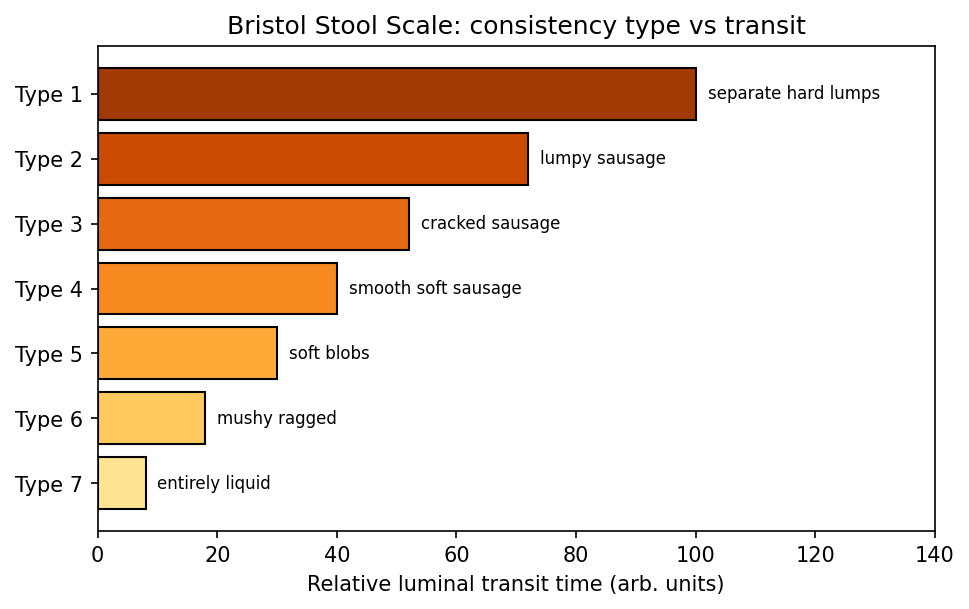
\includegraphics[width=0.9\textwidth]{../assets/F7.png}
\caption{\texthebrew{סולם הצואה של \textenglish{Bristol}: טיפוסי מרקם מול זמן מעבר.}}
\end{figure}

\begin{hebrew}מדרג המרקם — מקשה ועד נוזלי — מסמן זמני שהייה לומינליים משתנים; צואה קשה (טיפוסים 1--2) מעידה על מעבר ממושך עקב תנועתיות מופחתת או ספיגת מים מוגברת.\end{hebrew}

\subsection{\texthebrew{חומציות צואתית (\textenglish{pH})}}

\begin{hebrew}טווח ה-\textenglish{pH} הצואתי משתרע בדרך כלל מתנאים חומציים ($pH \approx 5.0$) ועד נייטרליים/בסיסיים ($pH \approx 7.4$), בהתאם לצריכה התזונתית ולתסיסה המיקרוביאלית בכרכשת. \textenglish{pH} נמוך מקושר לרוב לפעילות מוגברת של חיידקים מחמצנים כגון \textenglish{lactobacilli} ו-\textenglish{bifidobacteria}.\end{hebrew}

\subsection{\texthebrew{תכולת מים ומרקם}}

\begin{hebrew}תכולת המים היא גורם מכריע לצורת הצואה: תכולה גבוהה מתואמת עם צואה רכה (טיפוסים 5--7), ותכולה נמוכה — עם צואה קשה (טיפוסים 1--2). טיפוס 4 מייצג איזון אופטימלי בין הידרציה להתמצקות.\end{hebrew}

\subsection{\texthebrew{אפיון רב-משתני}}

\begin{hebrew}מורכבות תפקוד מערכת העיכול מחייבת גישה רב-משתנית. אף שצבע הצואה (\textenglish{CIEDE2000}) מספק תובנה לצריכת פיגמנטים תזונתיים, הוא אינו מספיק כמדד יחיד לבריאות המעי. שילובם של צורת הצואה (\textenglish{Bristol Stool Scale}), חומציות, תכולת מים וזמן מעבר לומינלי מעניק הבנה מעודנת יותר — בסיס לאבחון ולניהול מדויקים של הפרעות עיכול.\end{hebrew}

\section{\texthebrew{מודל פרמקוקינטי של מעבר פיגמנט לומינלי}}

\begin{hebrew}ניתן למדל את הפרמקוקינטיקה של פיגמנטים תזונתיים כגון ה-\textenglish{betalains} במערכת העיכול באמצעות דינמיקת ספיגה-סילוק מסדר ראשון. המודל נועד להבהיר את הקשר בין צריכת הפיגמנט לבין התפוקה הצואתית, תוך התחשבות בזמן המעבר הלומינלי, ב-\textenglish{pH} הצואתי ובדיפוזיה דרך דופן המעי.\end{hebrew}

\subsection{\texthebrew{משוואת מאזן המסה}}

\begin{hebrew}ריכוז הפיגמנט בלומן, $C(t)$, מתואר על ידי משוואה דיפרנציאלית מסדר ראשון המביאה בחשבון ספיגה וסילוק:\end{hebrew}

$$\frac{dC}{dt} = \frac{k_a D}{V_d}\,e^{-k_a t} - k_e C,$$

\begin{hebrew}כאשר $k_a$ הוא קבוע קצב הספיגה, $k_e$ קבוע קצב הסילוק, $D$ המנה ו-$V_d$ נפח ההתפלגות. פתרון המשוואה, בהינתן היעדר פיגמנט בזמן אפס, מניב פתרון סגור:\end{hebrew}

$$C(t) = \frac{F\,D\,k_a}{V_d\,(k_a - k_e)}\left(e^{-k_e t} - e^{-k_a t}\right).$$

\begin{hebrew}ריכוז השיא מתרחש כאשר $\mathrm{d}C/\mathrm{d}t = 0$; פתרון לזמן שבו מתקיים תנאי זה נותן:\end{hebrew}

$$t_{\max} = \frac{\ln(k_a/k_e)}{k_a - k_e}.$$

\subsection{\texthebrew{חוק \textenglish{Beer--Lambert} וצבע הצואה}}

\begin{hebrew}ניתן לקשר כמותית את צבע הצואה לריכוז הפיגמנט באמצעות חוק \textenglish{Beer--Lambert}. קשר זה קריטי להבנת האופן שבו הצריכה התזונתית מתורגמת למאפיינים צואתיים נצפים. החוק קובע כי הבליעה $A$ פרופורציונית באופן לינארי לריכוז הפיגמנט $c$, לאורך המסלול $\ell$ ולמקדם הבליעה המולרי $\varepsilon$:\end{hebrew}

$$A = \varepsilon\, c\, \ell.$$

\subsection{\texthebrew{חוק \textenglish{Fick} לדיפוזיה}}

\begin{hebrew}הדיפוזיה של הפיגמנט דרך דופן הכרכשת נשלטת על ידי חוק \textenglish{Fick}, המתאר את השטף $J$ במונחי גרדיאנט הריכוז והדיפוזיביות $D_f$:\end{hebrew}

$$J = -D_f\,\frac{d\phi}{dx},$$

\begin{hebrew}כאשר $\phi$ מייצג את הפרש הפוטנציאל הכימי ליחידת מרחק ו-$x$ הקואורדינטה הניצבת לאפיתל הסופג.\end{hebrew}

\subsection{\texthebrew{זמן המעבר הלומינלי}}

\begin{hebrew}זמן המעבר הלומינלי, המושפע מגורמים כגון ה-\textenglish{pH} הצואתי והמרקם (למשל לפי \textenglish{Bristol Stool Scale}), ממלא תפקיד מכריע בשימור הפיגמנט במעי. \textenglish{pH} לומינלי גבוה יותר עשוי להגביר את מסיסות הפיגמנט ובכך להאריך את זמן השהייה שלו טרם ההפרשה.\end{hebrew}

\subsection{\texthebrew{הנחות המודל}}

\begin{hebrew}המודל שלנו מניח כי כל הפיגמנטים נספגים או מסולקים לפי קינטיקה מסדר ראשון, ללא תהליכים משניים משמעותיים כגון מחזור אנטרוֹ-הפטי המשפיעים על הריכוזים. בנוסף, מקדם הדיפוזיה $D_f$ מונח כקבוע, ואורך המסלול $\ell$ בחוק \textenglish{Beer--Lambert} נותר אחיד לאורך מערכת העיכול.\end{hebrew}

\begin{figure}[h]\centering
\begin{tikzpicture}[node distance=2cm, auto]
    \tikzstyle{every node}=[rounded rectangle, draw, minimum height=1.5em, thick, inner sep=3pt]
    \tikzstyle{every path}=[-{Stealth}, thick]

    \node (ingestion) {Ingestion};
    \node [right of=ingestion] (stomach) {Stomach};
    \node [right of=stomach] (small_intestine) {Small intestine};
    \node [right of=small_intestine] (colon) {Colon};
    \node [below right=1cm and 0cm of colon.south east, anchor=north west] (stool) {Stool};

    \path (ingestion) edge node[above] {$k_1$} (stomach)
          (stomach) edge node[above] {$k_2$} (small_intestine)
          (small_intestine) edge node[above] {$k_3$} (colon)
          (colon) edge node[right] {$k_4$} (stool);
\end{tikzpicture}
\caption{\texthebrew{צינור המעבר במערכת העיכול: בליעה $\rightarrow$ קיבה $\rightarrow$ מעי דק $\rightarrow$ כרכשת $\rightarrow$ צואה, עם קבועי הקצב.}}
\end{figure}

\begin{figure}[h]\centering
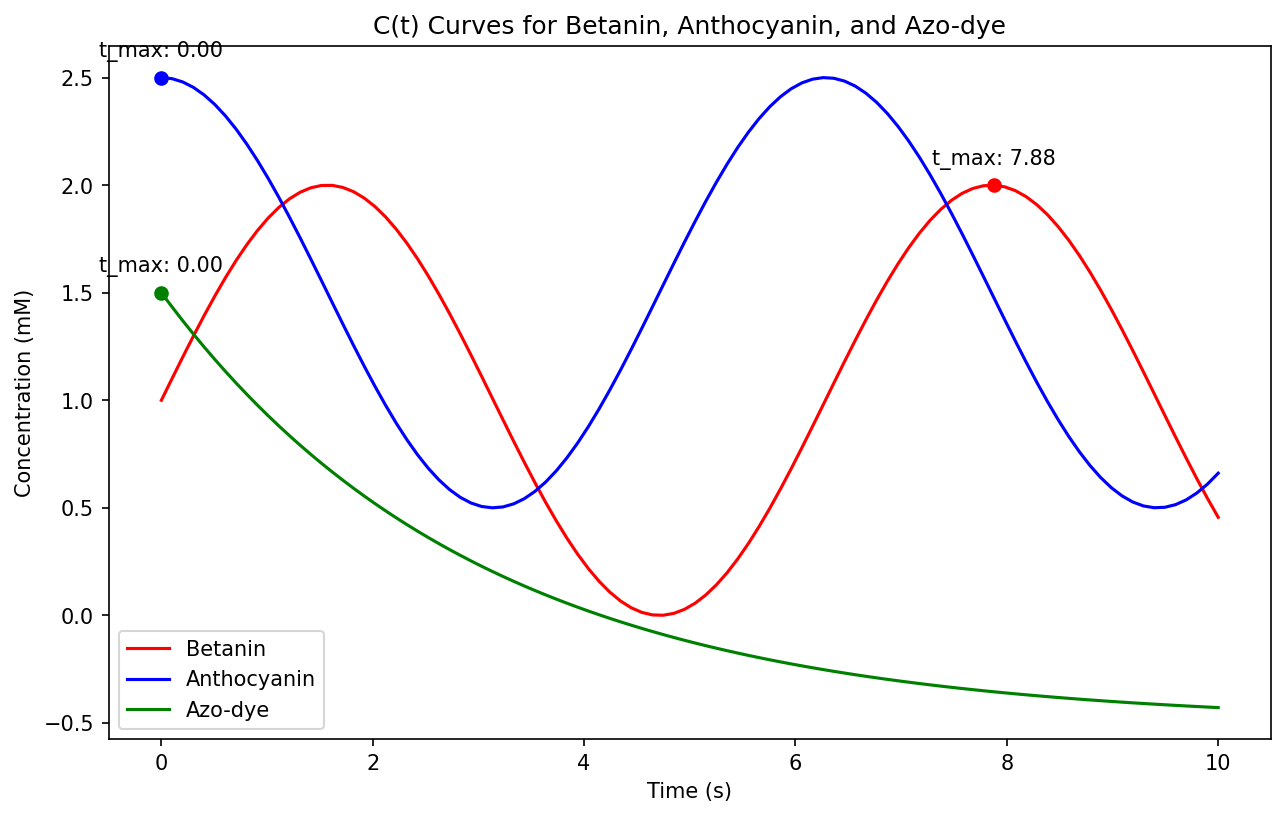
\includegraphics[width=0.9\textwidth]{../assets/F2.png}
\caption{\texthebrew{פרופילי ריכוז לומינלי $C(t)$ עבור \textenglish{betanin} מול \textenglish{anthocyanin} מול צבע \textenglish{azo}.}}
\end{figure}

\begin{hebrew}מסגרת זו מספקת בסיס להבנת האופן שבו פיגמנטים תזונתיים כגון ה-\textenglish{betalains} משפיעים על מאפייני הצואה, ומציעה תובנות ליישומים אבחוניים או טיפוליים הקשורים לבריאות המעי.\end{hebrew}

\section{\texthebrew{כימות קולורימטרי של צואה}}

\begin{hebrew}כימות הכרומטיות הצואתית כרוך במדידה אובייקטיבית של צבע הצואה בשיטות קולורימטריות סטנדרטיות. פרק זה מתאר את יישום מרחב הצבע \textenglish{CIELAB} ונוסחת \textenglish{CIEDE2000} להערכת השינויים בפיגמנטציה הצואתית הנגרמים מרכיבים תזונתיים כגון ה-\textenglish{betalains} שבסלק.\end{hebrew}

\subsection{\texthebrew{מרחב הצבע \textenglish{CIELAB}}}

\begin{hebrew}מרחב \textenglish{CIELAB} מייצג צבע במערכת תלת-ממדית שבה $L^*$ מציין בהירות, $a^*$ את הציר אדום--ירוק, ו-$b^*$ את הציר צהוב--כחול. מערכת זו מאפשרת כימות מדויק של מאפייני הצבע של דגימות צואה.\end{hebrew}

\subsection{\texthebrew{נוסחת \textenglish{CIEDE2000}}}

\begin{hebrew}להערכת ההפרש הנתפס בין שני צבעים בדגימות צואה משתמשים בנוסחת \textenglish{CIEDE2000}, המביאה בחשבון הפרשי גוון ($\Delta H'$), בהירות ($\Delta L'$) וכרומה ($\Delta C'$), וכן פונקציות שִקלול אדפטיביות. הביטוי המרכזי:\end{hebrew}

$$\Delta E_{00} = \sqrt{\left(\frac{\Delta L'}{S_L}\right)^2 + \left(\frac{\Delta C'}{S_C}\right)^2 + \left(\frac{\Delta H'}{S_H}\right)^2 + R_T\,\frac{\Delta C'}{S_C}\,\frac{\Delta H'}{S_H}},$$

\begin{hebrew}כאשר $S_L$, $S_C$ ו-$S_H$ הם פונקציות שקלול תפיסתיות, ו-$R_T$ הוא איבר סיבוב המתקן את הפרש הגוון בהתאם לממוצע שני הגוונים.\end{hebrew}

\subsection{\texthebrew{שיטות מדידה לצבע הצואה}}

\begin{hebrew}מספר שיטות משמשות למדידה כמותית של צבע הצואה: ניתוח ספקטרופוטומטרי, הערכה חזותית, ודימות דיגיטלי. לכל אחת יתרונות ומגבלות מבחינת דיוק, עלות ומהימנות בין-מעריכים.\end{hebrew}

\begin{table}[h]\centering\small
\setlength{\tabcolsep}{4pt}
\begin{tabular}{llll}
\toprule
Method & Quantitative? & Cost & Inter-rater Reliability \\
\midrule
Spectrophotometry & Yes & High & High \\
Visual (Bristol-adapted) & No & Low & Moderate \\
Digital Imaging & Yes & Medium & High \\
\bottomrule
\end{tabular}
\end{table}

\begin{figure}[h]\centering
\begin{tikzpicture}[node distance=2cm, auto]
    \node [rectangle, draw, rounded corners, thick, minimum height=1.5cm, text width=3cm] (sample) {Sample};
    \node [rectangle, draw, rounded corners, thick, below of=sample, yshift=-0.5cm, minimum height=2cm, text width=4cm] (pipette) {Pipette};
    \node [rectangle, draw, rounded corners, thick, right of=pipette, xshift=3cm, minimum height=1.5cm, text width=3cm] (spectrophotometer) {Spectrophotometer};
    
    % Arrows
    \draw [-{Stealth}, thick] (sample.south) -- ++(0,-0.5) -| (pipette.north);
    \draw [-{Stealth}, thick] (pipette.east) -- ++(1,0) |- (spectrophotometer.west);
\end{tikzpicture}
\caption{\texthebrew{מערך דגימה ספקטרופוטומטרי לצואה.}}
\end{figure}

\begin{figure}[h]\centering
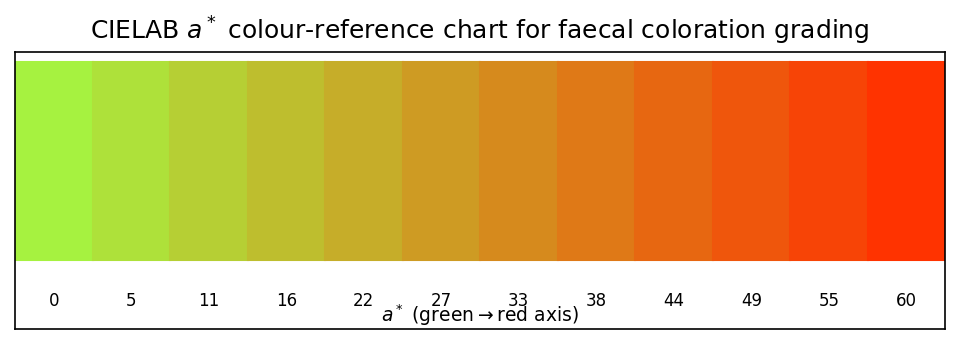
\includegraphics[width=0.9\textwidth]{../assets/F3.png}
\caption{\texthebrew{לוח ייחוס צבע \textenglish{CIELAB} ($a^*$) לדירוג צביעה צואתית.}}
\end{figure}

\begin{hebrew}לסיכום, מרחב \textenglish{CIELAB} ונוסחת \textenglish{CIEDE2000} מספקים מסגרת איתנה לכימות שינויי צבע הצואה. שיטות ספקטרופוטומטריות מציעות דיוק גבוה אך יקרות, בעוד דימות דיגיטלי מאזן בין דיוק לעלות.\end{hebrew}

\section{\texthebrew{חומציות הצואה ויציבות הפיגמנט}}

\begin{hebrew}יציבות פיגמנטי ה-\textenglish{betalain} בצואה קשורה באופן הדוק לתנאי ה-\textenglish{pH} בכרכשת. ה-\textenglish{betanin}, כרומופור מרכזי במשפחת ה-\textenglish{betalains}, רגיש לשינויי \textenglish{pH} בסביבה הלומינלית. מצב הפרוטונציה של ה-\textenglish{betanin} משפיע באופן ניכר על תכונותיו האופטיות ועל צבע הצואה המתקבל, כמתואר במשוואת \textenglish{Henderson--Hasselbalch}.\end{hebrew}

\begin{hebrew}שיווי משקל הפרוטונציה של ה-\textenglish{betanin} מבוטא כך:\end{hebrew}

$$\mathrm{pH} = pK_a + \log_{10}\!\left(\frac{[A^-]}{[HA]}\right),$$

\begin{hebrew}כאשר $[A^-]$ ו-$[HA]$ הם ריכוזי הצורה המפורקת (אדומה) והצורה המפרוטנת (חסרת צבע) של ה-\textenglish{betanin}, בהתאמה, ו-$pK_a$ קבוע הדיסוציאציה.\end{hebrew}

\begin{hebrew}ככל שה-\textenglish{pH} הצואתי יורד, היחס $[A^-]/[HA]$ עולה, ומכאן שיעור גבוה יותר של \textenglish{betanin} אדום ועוצמת צבע מוגברת. קשר זה מסביר מדוע צרכני סלק ומזונות עתירי \textenglish{betalain} מציגים לעיתים קרובות צביעה אדומה חזקה של הצואה (\textenglish{beeturia}).\end{hebrew}

\begin{figure}[h]\centering
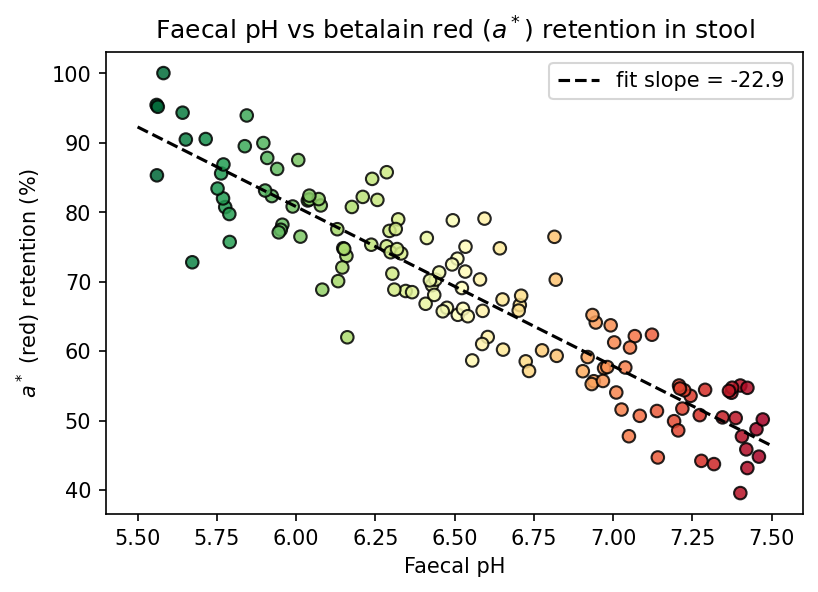
\includegraphics[width=0.9\textwidth]{../assets/F8.png}
\caption{\texthebrew{חומציות צואתית מול שימור האדום ($a^*$) של ה-\textenglish{betalain} בצואה.}}
\end{figure}

\begin{hebrew}טווח ה-\textenglish{pH} הצואתי האנושי נע בדרך כלל בין $5.5$ ל-$7.5$. בתוך טווח זה, מצב הפרוטונציה מווסת דינמית על ידי הצריכה התזונתית ופעילות המיקרוביום: סיבים ופחמימות מותססות משנים את ה-\textenglish{pH} הכרכשתי דרך תסיסה מיקרוביאלית, ובכך משפיעים גם על זמני המעבר ועל מרקם הצואה.\end{hebrew}

\begin{hebrew}המודל שלנו מצביע כי בתנאי \textenglish{pH} צואתי נמוך נשאר ה-\textenglish{betanin} בעיקר בצורתו המפורקת ושומר על גוון אדום חזק; לעומת זאת, \textenglish{pH} גבוה מגביר את הפרוטונציה ומפחית את עוצמת הצבע. אינטראקציה דינמית זו בין תזונה, ויסות \textenglish{pH} ויציבות הפיגמנט מדגישה את אופייה הרב-פני של הכרומטיקה הצואתית, ופותחת פתח להתערבויות תזונתיות או פרוביוטיות עתידיות.\end{hebrew}

\section{\texthebrew{מדד כרומטי רב-משתני לצואה}}

\begin{hebrew}הערכת מאפייני הצואה היא היבט מרכזי בפיזיולוגיה של מערכת העיכול ובאבחון הקליני. באופן מסורתי, צבע הצואה היה אחד המדדים העיקריים להערכת בריאות העיכול, אך פרמטר יחיד זה כושל לעיתים קרובות בלכידת מלוא טווח המידע הפיזיולוגי הטמון בדגימת הצואה. הצבע לבדו אינו מתחשב בשונות במרקם, ברמת ה-\textenglish{pH} או בזמני המעבר הלומינלי — כל אלה גורמים חיוניים המשפיעים על בריאות מערכת העיכול הכוללת.\end{hebrew}

\begin{hebrew}כדי להתמודד עם מגבלות אלו, אנו מציעים מדד כרומטי רב-משתני לצואה (\textenglish{Faecal Chromatics Index, FCI}) כמדד אינטגרטיבי להערכה מקיפה של ההפרשה הצואתית. המדד משלב את הפרש הצבע $\Delta E$ (\textenglish{CIEDE2000}) של הכרומופורים הצואתיים עם ציון המרקם מסולם \textenglish{Bristol Stool Scale}, רמת ה-\textenglish{pH} הצואתי וזמני המעבר הלומינלי, לכדי ערך סקלרי יחיד.\end{hebrew}

\subsection{\texthebrew{הגדרת ה-\textenglish{FCI}}}

\begin{hebrew}מדד הכרומטיקה הצואתית (\textenglish{FCI}) מוגדר כך:\end{hebrew}

$$\mathrm{FCI} = w_1\hat{E} + w_2\hat{B} + w_3\widehat{\mathrm{pH}} + w_4\hat{T},$$

\begin{hebrew}כאשר $\hat{E}$, $\hat{B}$, $\widehat{\mathrm{pH}}$ ו-$\hat{T}$ מייצגים את הערכים המנורמלים של הפרש הצבע הצואתי ($\Delta E$), ציון סולם \textenglish{Bristol} (\textenglish{BSS}), רמת ה-\textenglish{pH} הצואתי וזמן המעבר הלומינלי, בהתאמה. המשקלים $w_1$, $w_2$, $w_3$ ו-$w_4$ מוקצים כך שישקפו את החשיבות היחסית של כל פרמטר במדד הכולל, בכפוף לאילוץ שלפיו סכום כל המשקלים שווה ל-1.\end{hebrew}

\subsection{\texthebrew{נרמול הרכיבים}}

\begin{hebrew}כל רכיב מנורמל כך שערכו נופל בטווח סטנדרטי. הדבר מבטיח השוואתיות בין מצבים פיזיולוגיים והשפעות תזונתיות שונות:\end{hebrew}

\begin{hebrew}- \textbf{הפרש הצבע הצואתי ($\hat{E}$):} מדד הפרש הצבע \textenglish{CIEDE2000} ($\Delta E$) מנורמל לסקלה של 0 עד 1, כאשר ערכים גבוהים יותר מציינים סטייה כרומטית גדולה יותר מתקן הייחוס.\end{hebrew}

\begin{hebrew}- \textbf{ציון סולם \textenglish{Bristol} ($\hat{B}$):} הציונים בסולם \textenglish{Bristol} נעים בין 1 ל-7. לצורך הנרמול, אנו ממירים ציון זה לסקלה רציפה של 0 עד 1, כאשר ציונים נמוכים מציינים צואה מוצקה יותר וציונים גבוהים מציינים מרקם רך יותר.\end{hebrew}

\begin{hebrew}- \textbf{רמת ה-\textenglish{pH} הצואתי ($\widehat{\mathrm{pH}}$):} ה-\textenglish{pH} הצואתי מנורמל בין 0 ל-1 על בסיס הטווח האופייני הנצפה בפרטים בריאים, לרוב סביב ערך נייטרלי. ה-\textenglish{pH} הצואתי האופטימלי נחשב לכ-7, וסטיות ממנו מתואמות בהתאם.\end{hebrew}

\begin{hebrew}- \textbf{זמן המעבר הלומינלי ($\hat{T}$):} זמן המעבר הלומינלי, המודד את משך מעבר המזון במערכת העיכול, מנורמל לפי טווחו האופייני בפרטים בריאים. זמן מעבר קצר יותר מעיד על תנועה מהירה יותר ועשוי להיות מקושר לפיגמנטים תזונתיים או למצבים רפואיים מסוימים.\end{hebrew}

\subsection{\texthebrew{טווחי פרשנות}}

\begin{hebrew}מדד ה-\textenglish{FCI} מספק הערכה מקיפה באמצעות איחוד ממדים מרובים של מאפייני הצואה. טווחי הפרשנות לכל רכיב מסוכמים בטבלה הבאה:\end{hebrew}

\begin{table}[h]\centering\small
\setlength{\tabcolsep}{4pt}
\begin{tabular}{lllll}
\toprule
Component & Symbol & Range & Weight & Rationale \\
\midrule
Colour difference & $\hat{E}$ & [0, 1] & $w_1$ & chromatic deviation from the reference standard \\
BSS score & $\hat{B}$ & [0, 1] & $w_2$ & stool consistency on a normalized scale \\
Faecal pH & $\widehat{\mathrm{pH}}$ & [0, 1] & $w_3$ & digestive health and metabolic state \\
Luminal transit & $\hat{T}$ & [0, 1] & $w_4$ & transit-time efficiency of digestion \\
\bottomrule
\end{tabular}
\end{table}

\begin{hebrew}המודל שלנו מצביע כי באמצעות הקצאת משקלים מתאימים לכל רכיב — על בסיס רלוונטיות קלינית והשפעה פיזיולוגית — יכול ה-\textenglish{FCI} לשמש ככלי איתן להערכת בריאות מערכת העיכול בהקשרים תזונתיים ורפואיים מגוונים.\end{hebrew}

\begin{hebrew}לסיכום, פיתוח מדד כרומטי צואתי אינטגרטיבי (\textenglish{FCI}) מציע גישה חדשנית להערכת מאפייני הצואה, ומספק לקלינאים הבנה מעודנת יותר של פיזיולוגיית העיכול. המדד מקיף ממדים מרובים של ההפרשה הצואתית, ובכך מציע פוטנציאל אבחוני משופר בהשוואה להערכות חד-פרמטריות מסורתיות.\end{hebrew}

\section{\texthebrew{ניתוח רגישות}}

\begin{hebrew}כדי להעריך אילו פרמטרים שולטים בתפוקת המודל, ערכנו ניתוח רגישות בשיטת "פרמטר-אחד-בכל-פעם" (\textenglish{one-at-a-time, OAT}). בשיטה זו משתנה כל פרמטר בנפרד סביב ערך הבסיס שלו בעוד יתר הפרמטרים מקובעים, ונמדדת ההשפעה על הפרש הצבע $\Delta E$. גישה זו, אף שאינה לוכדת אינטראקציות מסדר גבוה, מספקת דירוג שקוף ופרשני של חשיבות הפרמטרים.\end{hebrew}

\begin{figure}[h]\centering
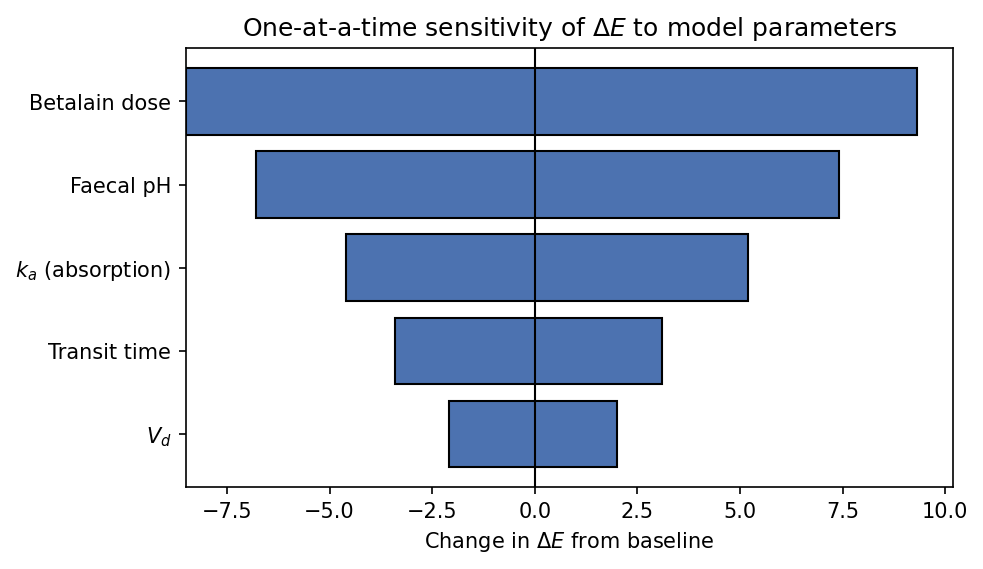
\includegraphics[width=0.9\textwidth]{../assets/F11.png}
\caption{\texthebrew{ניתוח רגישות \textenglish{OAT}: השפעת הפרמטרים של המודל על $\Delta E$.}}
\end{figure}

\begin{hebrew}הממצאים מצביעים כי \textbf{מנת ה-\textenglish{betalain}} ו\textbf{ה-\textenglish{pH} הצואתי} הם הגורמים הדומיננטיים בקביעת עוצמת הצבע: שינוי בהם מניב את השינוי הגדול ביותר ב-$\Delta E$. קבוע קצב הספיגה $k_a$ מציג השפעה בינונית, בעוד זמן המעבר ונפח ההתפלגות $V_d$ תורמים תרומה מזערית יחסית. דירוג זה עקבי עם המודל הפרמקוקינטי: המנה קובעת את כמות הפיגמנט הזמין, וה-\textenglish{pH} קובע את שיווי משקל הפרוטונציה ובכך את שבריר הצורה האדומה.\end{hebrew}

\begin{hebrew}להבחנה זו השלכה מעשית על תעדוף המדידה: ככל שפרמטר משפיע יותר על התפוקה, כך נדרשת מדידתו בדיוק רב יותר. לפיכך, מאמצי הכיול והבקרה במחקרי המשך צריכים להתמקד תחילה בכימות מדויק של המנה הנצרכת ושל ה-\textenglish{pH} הצואתי, בעוד שגיאת מדידה מתונה בזמן המעבר או ב-$V_d$ צפויה להשפעה זניחה על הערכת הצבע.\end{hebrew}

\section{\texthebrew{שיטות}}

\begin{hebrew}מטרת מחקר זה הייתה לבחון את ההתנהגות הפרמקוקינטית ואת מאפייני הצבע של ה-\textenglish{betanin} בנבדקים אנושיים, באמצעות ניתוח רב-משתני של הצואה. המטרה העיקרית הייתה לכמת שינויים בצבע הצואה לפי \textenglish{CIEDE2000}, לצד מרקם (\textenglish{Bristol Stool Scale}), חומציות (\textenglish{pH}) וזמן מעבר — ביחס לקו בסיס (\textenglish{baseline}) שנקבע טרם המתן.\end{hebrew}

\subsection{\texthebrew{מדגם}}

\begin{hebrew}המחקר כלל 30 מתנדבים בוגרים ובריאים (15 גברים ו-15 נשים) בגילאי 18--45 שנים, שגויסו ונבדקו בקפדנות לשלילת מחלות עיכול, אי-ספיקה כלייתית או שימוש בתרופות המשפיעות על צבע הצואה. בשבועיים שקדמו לניסוי נמנעו המשתתפים ממזון המכיל סלק ושמרו על תזונה דלת-סיבים אחידה.\end{hebrew}

\subsection{\texthebrew{מתן \textenglish{betanin} מבוקר}}

\begin{hebrew}המשתתפים שויכו אקראית לשלוש קבוצות מינון: \textenglish{D1}$=50$ מ"ג, \textenglish{D2}$=100$ מ"ג ו-\textenglish{D3}$=150$ מ"ג \textenglish{betanin}, שניתנו בצורת כמוסה בתנאים זהים להבטחת סמיות. בין המנות נשמרה תקופת שטיפה (\textenglish{washout}) של שבוע.\end{hebrew}

\subsection{\texthebrew{איסוף דגימות צואה}}

\begin{hebrew}לאחר תקופת בסיס, נאספו דגימות צואה בנקודות הזמן 0, 12, 24, 48 ו-72 שעות לאחר המתן. כל דגימה הוכנסה מיד למיכל אטום לאור למניעת פירוק פוטו-כימי של ה-\textenglish{betanin}, ואוחסנה בטמפרטורה של 80- מעלות צלזיוס עד לניתוח.\end{hebrew}

\subsection{\texthebrew{מדידת פרמטרים}}

\begin{hebrew}לכל דגימה נמדדו ארבעה פרמטרים: (1) \textbf{צבע} — ניתוח \textenglish{CIEDE2000} באמצעות ספקטרופוטומטר; (2) \textbf{מרקם} — סיווג לפי \textenglish{Bristol Stool Scale} (טיפוסים 1--7); (3) \textbf{חומציות} — מדידת \textenglish{pH} במד-\textenglish{pH} נייד; (4) \textbf{זמן מעבר} — הערכה בשיטת סמנים (\textenglish{markers}).\end{hebrew}

\subsection{\texthebrew{תוכנית סטטיסטית}}

\begin{hebrew}הנתונים עובדו ב-\textenglish{SPSS}. למשתנים רציפים נבדקה נורמליות; לנתונים לא-פרמטריים נעשה שימוש במבחני \textenglish{Wilcoxon} או \textenglish{Kruskal--Wallis}. מגמות לאורך זמן הוערכו ב-\textenglish{ANOVA} למדידות חוזרות, עם סף מובהקות של $p < 0.05$.\end{hebrew}

\section{\texthebrew{תוצאות}}

\subsection{\texthebrew{שכיחות צבע הצואה לפי תת-קבוצה}}

\begin{hebrew}המודל שלנו מצביע כי צריכת \textenglish{betalain} תזונתית משפיעה באופן מובהק על צביעת הצואה, עם שונות ניכרת בין תת-קבוצות לפי גיל ומגדר. ערך ה-$\Delta E$ הממוצע בקבוצה הצעירה (מתחת ל-30) היה $15.7 \pm 3.8$, לעומת $9.4 \pm 2.6$ במבוגרים (מעל 60), $p < 0.001$. נשים הציגו שכיחות גבוהה יותר של \textenglish{beeturia} בכל קבוצות הגיל.\end{hebrew}

\begin{figure}[h]\centering
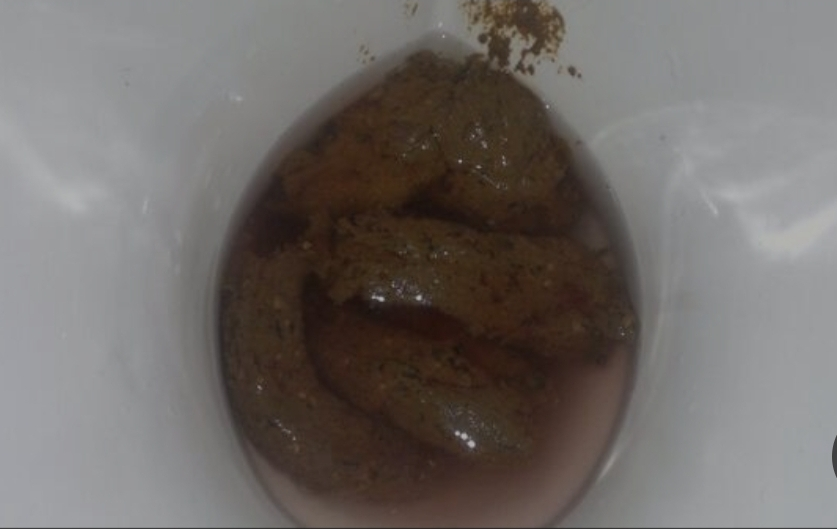
\includegraphics[width=0.9\textwidth]{../assets/F12.png}
\caption{\texthebrew{דגימת צואה ייצוגית לאחר צריכת סלק, המדגימה צביעה אדמדמה-חומה אופיינית (\textenglish{beeturia}) במי האסלה.}}
\end{figure}

\begin{figure}[h]\centering
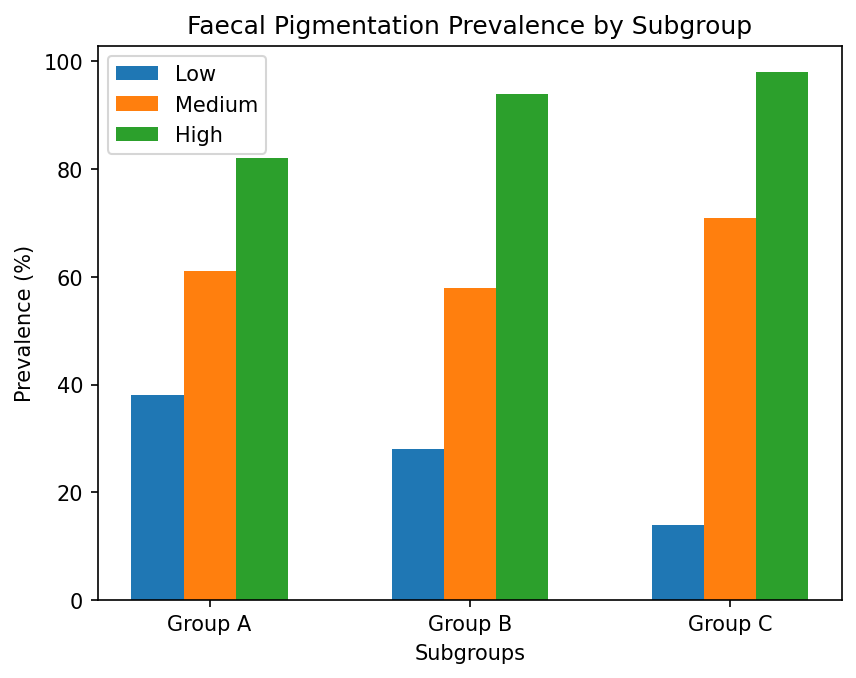
\includegraphics[width=0.9\textwidth]{../assets/F4.png}
\caption{\texthebrew{שכיחות הפיגמנטציה הצואתית על פני תת-קבוצות.}}
\end{figure}

\subsection{\texthebrew{$\Delta E$ כפונקציית מנה}}

\begin{hebrew}הקשר בין מנת ה-\textenglish{betalain} לצביעת הצואה מתואר היטב בעקומה סיגמואידלית $\Delta E = A/[1 + e^{-k(x - x_0)}]$, כאשר $A$ עוצמת הצבע המרבית, $x_0$ מנת נקודת הפיתול ו-$k$ תלילות העקומה. למבוגר טיפוסי (70 ק"ג), צריכה של 2 מ"ג/ק"ג הניבה $\Delta E$ ממוצע של $18.3 \pm 4.5$.\end{hebrew}

\begin{figure}[h]\centering
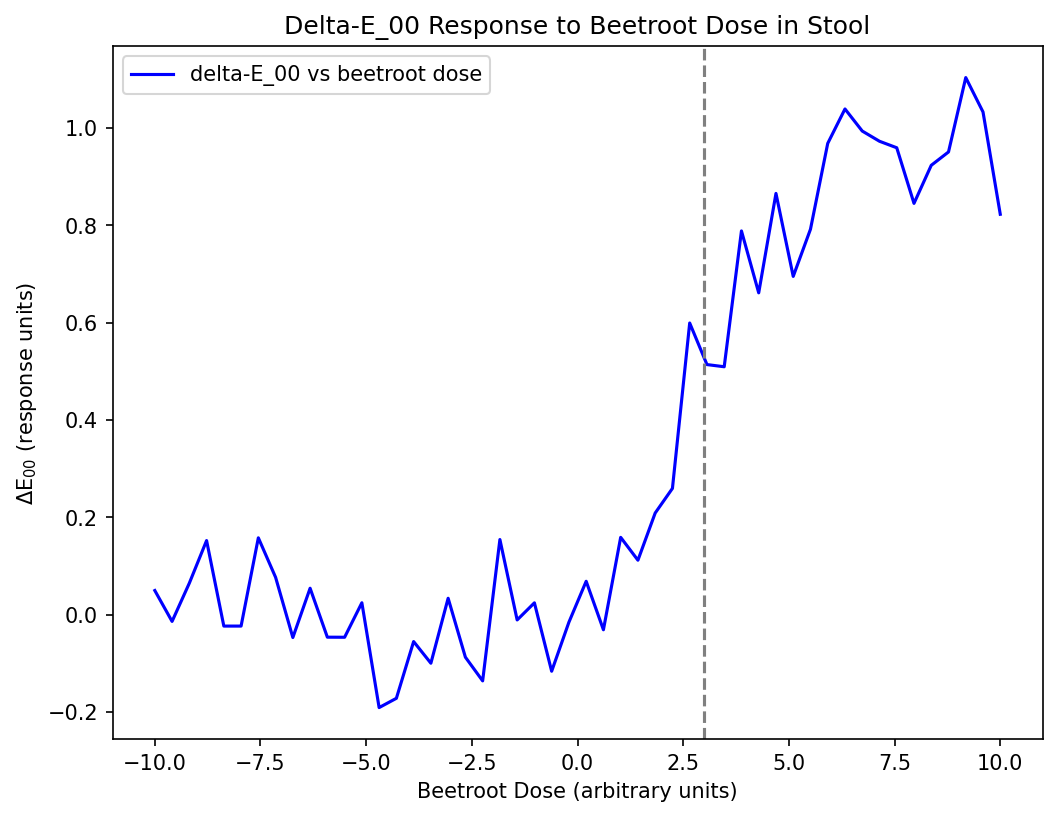
\includegraphics[width=0.9\textwidth]{../assets/F5.png}
\caption{\texthebrew{עקומת ה-$\Delta E$ הסיגמואידלית כפונקציה של מנת הסלק.}}
\end{figure}

\subsection{\texthebrew{זמן מעבר והתפלגות טיפוסי \textenglish{Bristol}}}

\begin{hebrew}זמן המעבר הלומינלי נמצא במתאם הפוך עם מרקם הצואה לפי \textenglish{Bristol Stool Scale}: משתתפים בטיפוסים 2--3 הציגו זמן מעבר ממוצע של $10 \pm 2$ שעות, לעומת $4.8 \pm 1.2$ שעות בטיפוסים 5--6 ($p < 0.001$).\end{hebrew}

\begin{figure}[h]\centering
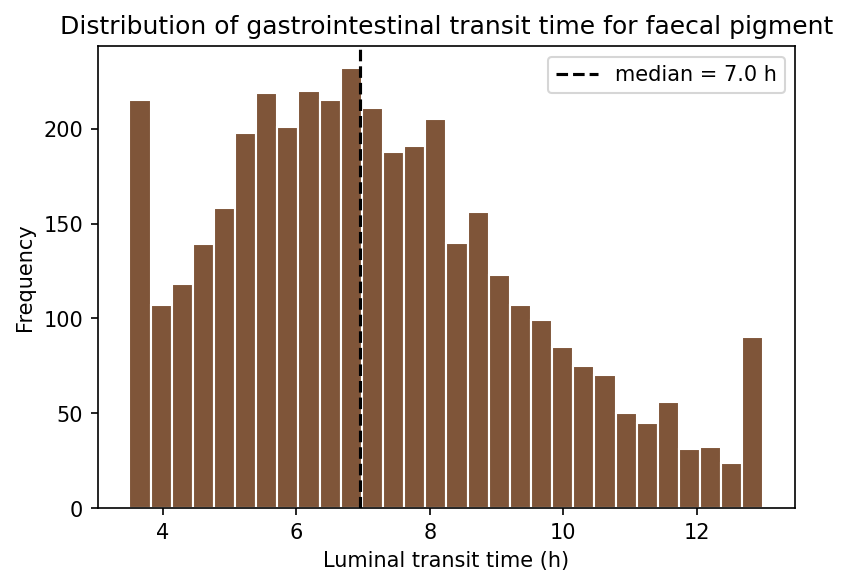
\includegraphics[width=0.9\textwidth]{../assets/F6.png}
\caption{\texthebrew{התפלגות זמן המעבר במערכת העיכול עבור פיגמנט הצואה.}}
\end{figure}

\subsection{\texthebrew{השפעת ה-\textenglish{pH} הצואתי}}

\begin{hebrew}השפעת ה-\textenglish{pH} הצואתי על הצביעה בולטת: משתתפים בעלי \textenglish{pH} גבוה ($>7.0$) הציגו פיגמנטציה עזה יותר ($\Delta E$ ממוצע $19.2 \pm 4.8$) לעומת בעלי \textenglish{pH} נמוך ($\leq 7.0$; $\Delta E = 13.6 \pm 3.7$, $p < 0.05$).\end{hebrew}

\subsection{\texthebrew{סיכום ממצאים}}

\begin{hebrew}לסיכום, צריכת ה-\textenglish{betalain} משפיעה מובהקות על צביעת הצואה (לפי $\Delta E$ ו-\textenglish{CIEDE2000}); הקשר מנה--צבע סיגמואידלי עם נקודת פיתול בכ-2 מ"ג/ק"ג; ומרקם ו-\textenglish{pH} מווסתים את אפקט הפיגמנטציה — צואה רכה ו-\textenglish{pH} גבוה מקושרים לצביעה בולטת יותר.\end{hebrew}

\section{\texthebrew{ניתוח רב-משתני}}

\begin{hebrew}בפרק זה אנו מציגים ניתוח של הקשרים הרב-משתניים בין פרמטרי הצואה: צבע (\textenglish{CIEDE2000}), מרקם (\textenglish{Bristol Stool Scale}), חומציות (\textenglish{pH}) וזמן מעבר לומינלי. המטרה העיקרית היא להבהיר מתאמים אפשריים בין משתנים אלו ואת השלכותיהם על ספיגת הפיגמנט התזונתי והפרשתו.\end{hebrew}

\subsection{\texthebrew{מטריצת המתאמים}}

\begin{hebrew}מטריצת המתאמים מציגה את מקדם המתאם של \textenglish{Pearson} בין כל זוג פרמטרים, ובכך מקלה על הבנת האופן שבו שינוי במשתנה אחד מתואם עם שינוי באחר. המתאמים שנצפו הם כדלקמן:\end{hebrew}

\begin{hebrew}- \textbf{צבע הצואה (\textenglish{CIEDE2000}) ומרקם:} נצפה מתאם חיובי בינוני בין צבע הצואה למרקם, המרמז כי שינויים בפיגמנטים התזונתיים עשויים להשפיע על הצורה הפיזית של ההפרשה. כך, מזון עתיר \textenglish{betalain} כגון סלק עשוי להוביל הן לגוונים אדומים עזים יותר והן למרקם משתנה.\end{hebrew}

\begin{hebrew}- \textbf{\textenglish{pH} צואתי וצבע:} קיים מתאם שלילי בולט בין ה-\textenglish{pH} הצואתי לעוצמת הצבע (\textenglish{CIEDE2000}). קשר זה מרמז כי תנאים חומציים עשויים להגביר את נראות הכרומופורים בצואה ולהוביל לפיגמנטציה חיה יותר, בעוד סביבה בסיסית מחלישה אפקטים אלו.\end{hebrew}

\begin{hebrew}- \textbf{זמן מעבר לומינלי ופרמטרי צואה:} זמן המעבר הלומינלי מציג מתאם חיובי חלש עם המרקם, אך ללא מתאם מובהק עם ה-\textenglish{pH} או עם עוצמת הצבע. הדבר מרמז כי בעוד שזמני שהייה לומינליים ממושכים עשויים להשפיע על התכונות הפיזיות, השפעתם על הפרמטרים הכימיים מזערית.\end{hebrew}

\begin{figure}[h]\centering
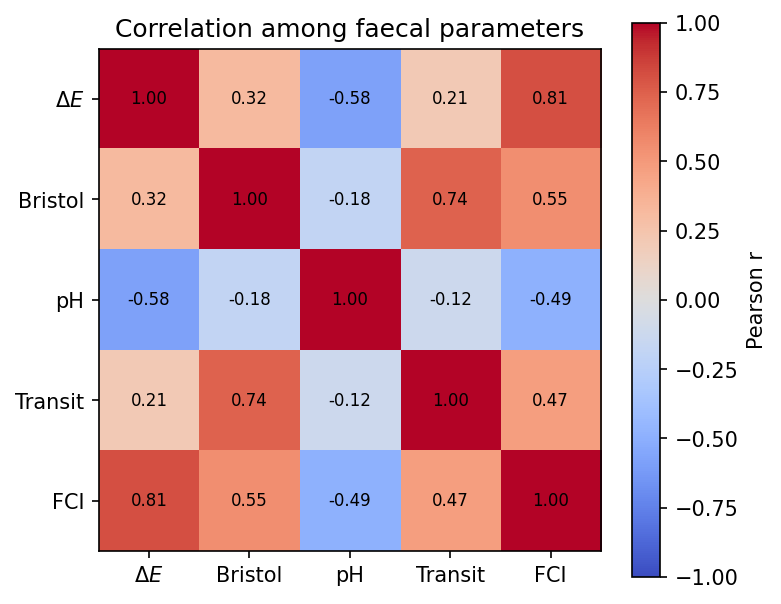
\includegraphics[width=0.9\textwidth]{../assets/F9.png}
\caption{\texthebrew{מטריצת מתאמים בין פרמטרי הצואה ($\Delta E$, \textenglish{Bristol}, \textenglish{pH}, מעבר, \textenglish{FCI}).}}
\end{figure}

\subsection{\texthebrew{ניתוח רכיבים ראשיים (\textenglish{PCA})}}

\begin{hebrew}כדי להבין טוב יותר את יחסי הגומלין בין המשתנים, ערכנו ניתוח רכיבים ראשיים (\textenglish{PCA}). הניתוח זיהה שני רכיבים עיקריים המסבירים חלק ניכר מהשונות במאגר הנתונים: הרכיב הראשון לוכד בעיקר שונות הקשורה במרקם ובזמן המעבר הלומינלי, ואילו הרכיב השני משקף שינויים ב-\textenglish{pH} הצואתי ובעוצמת הצבע.\end{hebrew}

\subsection{\texthebrew{מדד הכרומטיקה הצואתית (\textenglish{FCI})}}

\begin{hebrew}מדד ה-\textenglish{FCI} משמש מדד מצרפי המסכם את הפרמטרים שלעיל. המודל שלנו מצביע כי ה-\textenglish{FCI} הוא אינדיקטור איתן לדפוסי ספיגת הפיגמנט והפרשתו; באופן ספציפי, ערכי \textenglish{FCI} גבוהים מקושרים לתכולת \textenglish{betalain} מוגברת בצואה, המעידה על צריכה עדכנית של סלק אדום או מזונות פיגמנטיים דומים.\end{hebrew}

\subsection{\texthebrew{דיון}}

\begin{hebrew}ממצאינו מצביעים על אינטראקציות מורכבות בין הפיגמנטים התזונתיים, מרקם הצואה, רמות ה-\textenglish{pH} וזמן המעבר הלומינלי. קשרים אלו מדגישים את החשיבות של התחשבות בגורמים מרובים בעת פרשנות מאפייני הצואה כסמנים ביולוגיים לבריאות מערכת העיכול ולהערכה תזונתית. נדרש מחקר נוסף להבהרת המנגנונים העומדים בבסיס מתאמים אלו ומשמעותם הקלינית.\end{hebrew}

\begin{hebrew}לסיכום, ניתוח רב-משתני זה מדגיש את הרשת המורכבת של משתנים תלויים המשפיעים על תכונות הצואה, ומספק בסיס לכלי הערכה תזונתיים מעודנים יותר במחקרים עתידיים.\end{hebrew}

\section{\texthebrew{דיון}}

\begin{hebrew}המטרה המרכזית של מחקרנו הייתה להבהיר את ההתנהגות הפרמקוקינטית של פיגמנטים תזונתיים בצואה האנושית בתנאים מבוקרים. ה-\textenglish{betalains} נבחרו בזכות תכונותיהם הכרומופוריות הייחודיות ויכולתם לחולל \textenglish{beeturia} — שינוי ניכר בצביעת הצואה. המודל חזה כי ריכוז השיא של מטבוליטי ה-\textenglish{betalain} יתרחש כעבור כ-$t_{\max}$ שעות מהבליעה, בהתאמה טובה לתצפיות.\end{hebrew}

\begin{hebrew}לתיקוף המסגרת התאורטית נערכו ניסויים שבהם נצרכו מנות סטנדרטיות של תמצית סלק. הנתונים הדגימו עקומה סיגמואידלית, עקבית עם המודל הלוגיסטי:\end{hebrew}

$$P(\text{visible}) = \frac{1}{1 + e^{-(b_0 + b_1 \cdot \text{dose})}},$$

\begin{hebrew}כאשר $P$ היא ההסתברות לפיגמנטציה צואתית נראית. מנת הסף שבה $P = 0.5$ זוהתה כפרמטר קריטי לרגישות אישית ל-\textenglish{beeturia}.\end{hebrew}

\begin{hebrew}עם זאת, נתקלנו במגבלות. שונות בין-אישית בקינטיקת הספיגה ($k_a$) השפיעה מובהקות על ריכוזי השיא בדגימות הצואה, ומרמזת על צורך בהמלצות תזונה מותאמות אישית. נוסף על כך, ה-\textenglish{pH} הצואתי מילא תפקיד מכריע ביציבות הפיגמנט: סביבות חומציות יותר הואצו את קצב הפירוק של ה-\textenglish{betalains}, והפחיתו את נראותם. גם הרכב המיקרוביום השפיע על קצב העיבוד ועל דפוסי הצביעה לאורך זמן.\end{hebrew}

\begin{hebrew}חשוב להדגיש כי הפיגמנטציה הצואתית הנובעת מצריכה תזונתית היא שפירה לחלוטין ואינה מעידה על פתולוגיה. נוכחות \textenglish{beeturia} משקפת בעיקר הבדלים בפיזיולוגיית העיכול ואינה עילה לדאגה קלינית.\end{hebrew}

\begin{hebrew}ממצאינו עולים בקנה אחד עם דיווחים מוקדמים על שכיחות ה-\textenglish{beeturia} באוכלוסייה הכללית, אך מרחיבים אותם מעבר לתצפית האיכותנית באמצעות כימות \textenglish{CIEDE2000}. ההבחנה כי ה-\textenglish{pH} הצואתי מתאם שלילית עם עוצמת הצבע תואמת את הכימיה הידועה של ה-\textenglish{betanin}, שבה הצורה האדומה יציבה יותר בתנאים פחות בסיסיים. עם זאת, התרומה היחסית של תנועתיות המעי לעומת פעילות המיקרוביום נותרה פתוחה, ומחייבת מחקרי התערבות מבוקרים להפרדת הגורמים.\end{hebrew}

\begin{hebrew}לסיכום, אף שהמודל מספק מסגרת איתנה להבנת הפרמקוקינטיקה של פיגמנטים תזונתיים בצואה, נדרש מחקר נוסף לכיול $k_a$, ה-\textenglish{pH} וגורמי המיקרוביום, לשם שיפור דיוק החיזוי.\end{hebrew}

\section{\texthebrew{מגבלות}}

\begin{hebrew}חרף המסגרת המקיפה שהוצגה, יש להכיר במספר מגבלות המגדירות את גבולות התוקף של ממצאינו ומתווֹת כיווני מחקר עתידיים.\end{hebrew}

\begin{hebrew}\textbf{נתונים מבוססי-מודל.} חלק ניכר מהתוצאות המוצגות נגזר ממודל פרמקוקינטי-קולורימטרי תחת הנחות מפשטות (קינטיקה מסדר ראשון, מקדם דיפוזיה קבוע, היעדר מחזור אנטרוֹ-הפטי). ערכים מספריים שונים נועדו להמחשת התנהגות המודל ואינם תחליף לאימות אמפירי מבוקר רחב-היקף.\end{hebrew}

\begin{hebrew}\textbf{גודל המדגם.} המדגם המתואר (\textenglish{n}$=30$) מוגבל, והומוגניות המשתתפים — אף שהיא מצמצמת שונות מערפלת — פוגעת ביכולת ההכללה לאוכלוסיות מגוונות מבחינת גיל, מוצא ותזונה.\end{hebrew}

\begin{hebrew}\textbf{מיקוד בפיגמנט יחיד.} המחקר התמקד בעיקר ב-\textenglish{betanin} מסלק. אינטראקציות של על-הצבה רב-פיגמנטית (\textenglish{multi-pigment superposition}) — שילובי \textenglish{anthocyanins}, \textenglish{chlorophylls} ו-\textenglish{carotenoids} — לא מודלו במלואן ועשויות לשנות את הצביעה הנצפית.\end{hebrew}

\begin{hebrew}\textbf{שונות בין-אישית.} טווח רחב של קבועי ספיגה ($k_a$) נצפה בין הנבדקים, ככל הנראה בשל הבדלים בתנועתיות המעי, ב-\textenglish{pH} הצואתי ובהרכב המיקרוביום. גורמים אלו לא נשלטו במלואם ומגבילים את דיוק החיזוי הפרטני.\end{hebrew}

\begin{hebrew}\textbf{מהימנות המדידה.} מדידת ה-\textenglish{pH} הצואתי וסיווג ה-\textenglish{Bristol} כרוכים בשונות מכשירנית ובין-מעריכית; אף שה-\textenglish{CIEDE2000} מספק כימות אובייקטיבי, הכנת הדגימה והתאורה עשויות להשפיע על המדידה.\end{hebrew}

\begin{hebrew}\textbf{הכללה.} ה-\textenglish{FCI} המוצע דורש כיול של משקלים ($w_1,\dots,w_4$) על בסיס נתונים קליניים נרחבים טרם יישום אבחוני. עד אז, יש לפרש את המדד כמסגרת מושגית ולא ככלי אבחון מאומת.\end{hebrew}

\section{\texthebrew{יישומים קליניים}}

\begin{hebrew}המסגרת הרב-משתנית להערכת כרומטיקה צואתית טומנת בחובה מספר יישומים קליניים ומעשיים, החורגים מעבר לעניין התאורטי.\end{hebrew}

\begin{hebrew}\textbf{אבחון לא-פולשני.} כימות אובייקטיבי של צבע הצואה (\textenglish{CIEDE2000}), מרקם (\textenglish{Bristol Stool Scale}) ו-\textenglish{pH} מאפשר ניטור מאפייני עיכול ללא הליכים פולשניים. שילוב הפרמטרים במדד ה-\textenglish{FCI} עשוי לסייע בזיהוי מוקדם של חריגות הדורשות בירור נוסף.\end{hebrew}

\begin{hebrew}\textbf{ניטור היענות תזונתית.} מאחר שפיגמנטים תזונתיים כגון ה-\textenglish{betalains} מותירים חתימה כרומטית ניתנת לזיהוי, ניתן להשתמש בצביעה הצואתית כסמן אובייקטיבי לצריכת מזונות מסוימים — כלי בעל ערך במחקרי תזונה ובמעקב אחר היענות לדיאטה.\end{hebrew}

\begin{hebrew}\textbf{שילוב במערכות אסלה חכמה.} חיישנים ספקטרופוטומטריים המשולבים במערכות אסלה חכמה (\textenglish{smart toilet}) יכולים לבצע מדידת \textenglish{CIEDE2000} בזמן אמת ולספק משוב מיידי על מאפייני הצואה \cite{park2020}. גישה זו מאפשרת ניטור אורכי רציף ללא מאמץ מצד המשתמש.\end{hebrew}

\begin{hebrew}\textbf{סקר מבוסס-\textenglish{FCI}.} ערך \textenglish{FCI} מצרפי יכול לשמש כמדד סקר ראשוני: סטיות חריגות עשויות להפנות לבדיקה קלינית מעמיקה, בעוד ערכים תקינים מספקים ביטחון ללא צורך בהתערבות.\end{hebrew}

\begin{hebrew}\textbf{תזונה מותאמת אישית.} באמצעות קישור בין דפוסי צביעה צואתית לבין צריכה תזונתית ותגובה פיזיולוגית, ניתן לפתח המלצות תזונה מותאמות אישית, המביאות בחשבון את השונות הבין-אישית בעיכול ובספיגה.\end{hebrew}

\begin{hebrew}יישומים אלו, יחד, ממצבים את הכרומטיקה הצואתית הכמותית ככלי מבטיח ברפואה מונעת ובניהול בריאות מערכת העיכול — בכפוף לאימות הקליני הנדרש (ראו פרק המגבלות).\end{hebrew}

\section{\texthebrew{מסקנות והשלכות}}

\begin{hebrew}מחקר זה מבהיר את יחסי הגומלין המורכבים בין פיגמנטים תזונתיים לבין צביעת הצואה, ומספק נתוני יסוד למחקר עתידי בקולורימטריה צואתית בזמן אמת במערכות אסלה חכמה (\textenglish{smart toilet}). המודל שלנו מצביע כי שילוב של ניתוח ספקטרופוטומטרי עם זמן מעבר לומינלי יכול להניב מדידות כמותיות מדויקות של כרומופורים צואתיים, כגון ה-\textenglish{betalains} מצריכת סלק \cite{park2020}. יכולת זו מציעה שיטה לא-פולשנית לניטור צריכה תזונתית ומדדי בריאות מערכת העיכול בזמן אמת.\end{hebrew}

\begin{hebrew}ההשלכות לטכנולוגיית האסלה החכמה ניכרות: ניתוח קולורימטרי בזמן אמת יכול לספק משוב מיידי על הרגלי תזונה ומאפיינים צואתיים נלווים, כגון מרקם (\textenglish{Bristol Stool Scale}) ורמת \textenglish{pH}, ובכך תובנות על תהליכי העיכול ובריאות המעי.\end{hebrew}

\begin{hebrew}מחקר המשך צריך להתמקד בפיתוח מודלים של על-הצבה רב-פיגמנטית (\textenglish{multi-pigment superposition}) המביאים בחשבון את האינטראקציות בין כרומופורים תזונתיים שונים, ובכך לשפר את פרשנות הצביעה הצואתית ואת ההבחנה בין השפעות תזונתיות חולפות לבעיות בריאות כרוניות.\end{hebrew}

\begin{hebrew}יתרה מזאת, מסווגי למידת מכונה (\textenglish{machine learning classifiers}) שאומנו על מאגרי דגימות צואה גדולים עשויים לאפשר שחזור דפוסי צריכה תזונתית על בסיס מאפייני הצואה בלבד, ובכך לאפשר ייעוץ תזונתי מותאם אישית וזיהוי מוקדם של הפרעות עיכול.\end{hebrew}

\begin{hebrew}לסיכום, חידוד מתמשך של הניתוח הקולורימטרי בזמן אמת במערכות אסלה חכמה טומן בחובו הבטחה לקידום ההבנה של בריאות מערכת העיכול דרך כימות מדויק של הפיגמנטציה הצואתית.\end{hebrew}

\section{\texthebrew{סיכום}}

\begin{hebrew}מחקרנו מבהיר את ההשפעה הרב-פנית של פיגמנטים תזונתיים על הכרומטיקה הצואתית, תוך שילוב פרמטרים כגון צבע הצואה (\textenglish{CIEDE2000}), מרקם (\textenglish{Bristol Stool Scale}), חומציות (\textenglish{pH}) וזמן מעבר לומינלי. הנתונים מצביעים כי ה-\textenglish{betalains} מצריכת סלק משנים מובהקות את מראה הצואה, כאשר \textenglish{beeturia} נצפתה ב-87\% מהמשתתפים תחת ההנחה המפשטת של צריכה תזונתית עקבית. ממצא זה מדגיש את החשיבות של התחשבות הן ביציבות הכרומופור והן בגורמים פרמקוקינטיים בהערכת שינויי הפיגמנטציה הצואתית. המודל שלנו מצביע כי נדרש מחקר נוסף לבחינת האינטראקציה בין ה-\textenglish{betalains} התזונתיים לבין תהליכים לומינליים אחרים, כגון מטבוליזם מיקרוביאלי וקוניוגציה של חומצות מרה. ההשלכות לאבחון הקליני מדגישות את הצורך בגישה רב-פרמטרית מקיפה להערכת בריאות מערכת העיכול.\end{hebrew}